% Input common header
\documentclass[xcolor=dvipsnames]{beamer}

\usecolortheme[named=Blue]{structure}
\setbeamertemplate{itemize items}[circle]

\usepackage{smartdiagram}


\author{Dr. Paul Larsen}
\date{\today}



\title{Discrete Geometry for Risk and AI}
\begin{document}
\maketitle


\begin{frame}
\frametitle{Why discrete geometry?}

\begin{itemize}
\item Recent history: Dissatisfaction with deep learning, only ``curve fitting'', alternatives via \emph{causal graphical models} \cite{pearl2019limitations}
\item Less recent history: graphical models among first non-rules based AI approaches \cite{darwiche2009modeling}
\item Geometrical formulations of statistical objects, e.g. graphical models and probability polytopes\newline
\end{itemize}

\end{frame}


\begin{frame}
  \frametitle{Directed graphical model: university admission gender bias}
  \framesubtitle{Simpson paradox preview}

  \begin{figure}[ht]
    \centering
            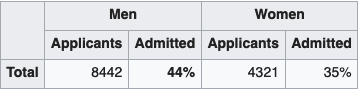
\includegraphics[height=0.15\textwidth]{graphics/berkeley} 
            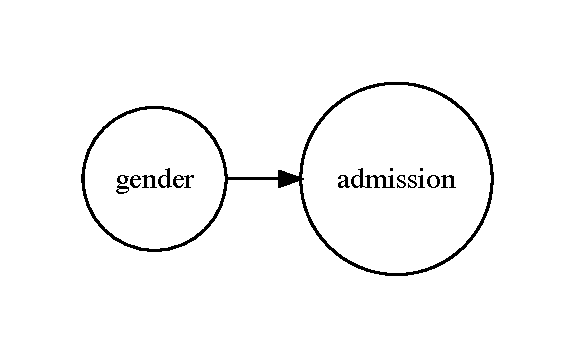
\includegraphics[height=0.4\textwidth]{graphics/admission_original}
       
    \end{figure}
    Sources: \cite{simpson-wikipedia} \cite{freedman1998statistics}
\end{frame}

\begin{frame}
  \frametitle{Bayesian networks: university admission gender bias}
  \framesubtitle{Simpson paradox preview}

  \begin{figure}[ht]
    \centering
            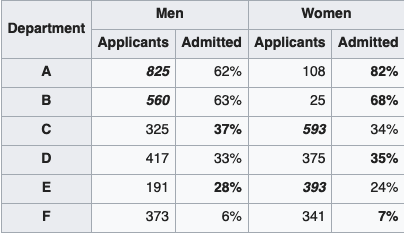
\includegraphics[height=0.35\textheight]{graphics/berkeley_later} 
            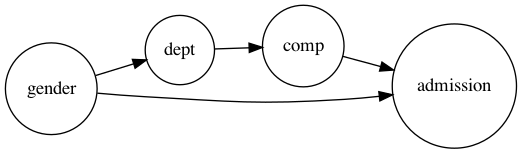
\includegraphics[height=0.35\textheight]{graphics/admission_later}
    \end{figure}
    Sources: \cite{simpson-wikipedia} \cite{Bickel398}
\end{frame}


\begin{frame}
\frametitle{Directed graphical model: hit rate for insurance quotes}
\begin{itemize}
  \item product type: financial, liability, property
  \item days: number of days to generate quote
  \item rating: measure of premium paid expected claims
  \item hit: 0 if quote refused, 1 if accepted
\end{itemize}
\begin{figure}[ht]
  \centering
  \includegraphics[height=0.7\textheight]{graphics/hit}
\end{figure}
\end{frame}


\begin{frame}
\frametitle{Undirected graphical model: credit default risk \cite{filiz2012graphical}}

\begin{itemize}
  \item Nodes take values 0 (healthy) or 1 (default)
  \item Industry nodes connect to other industry nodes
  \item Individual firm nodes connect only to corresponding industry node
\end{itemize}
\begin{figure}[ht]
  \centering
  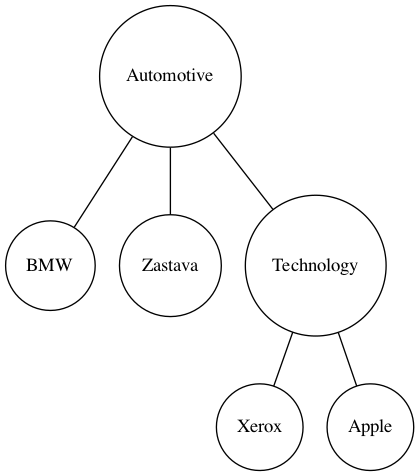
\includegraphics[height=0.6\textheight]{graphics/credit_default}
\end{figure}
\end{frame}


\begin{frame}
\frametitle{Graph definitions}
\begin{definition}
A \emph{graph} is a pair of sets $(V, E)$, where $V$ is called the set of \emph{vertices} (or \emph{nodes}) and $E$ is called the set of \emph{edges}, such that the set of edges corresponds injectively to pairs of vertices. \newline
\end{definition}

\emph{Notes}
\begin{itemize}
\item Typically `pairs of vertices` does not include self-pairs, but this can be relaxed, leading to graphics with with loops.
\item The injectivity requirement can also be relaxed, leading to \emph{multigraphs}.
\end{itemize}
\end{frame}


\begin{frame}
\frametitle{Graphical models}
\begin{definition}
(Informal) A graphical model is a graph whose nodes represent variables and whose edges represent direct statistical dependencies between the variables.\newline
\end{definition}

\emph{Why graphical models?}
\begin{itemize}
\item For probability distributions admitting a graphical model representation, then graph properties (\emph{d-separation}) imply conditional independence relations.
\item Conditional independence relations reduce the number of parameters required to specify a probability distribution.
\item Graphical models come in two flavors depending on their edges: directed (aka \emph{Bayesian Networks}) and undirected (aka \emph{random Markov fields}.
\end{itemize}
\end{frame}


\begin{frame}
\frametitle{Directed acyclic graphs}

\begin{definition}
A graph $G = (V, E)$ is a \emph{directed acyclic graph} (denoted also \emph{DAG}) if all edges have an associated direction, and no edge path consistent with the directions forms a cycle.\newline

If there is a directed path from $X_i$ to $X_j$, then $X_i$ is called a \emph{parent} of $X_j$, and $Pa(X_j) \subseteq V$ is the set of all parents of $X_j$.
\end{definition}

\begin{definition}
  If $X = (X_1, \ldots, X_m)$ admits a DAG $G$, then $X_G$ is a \emph{DAG model} if the distribution of $X$ decomposes according to $G$, i.e.

  \begin{equation*}
    P(X) = \prod_{i \in \{1, \ldots, m\}} P(X_i | Pa(X_i))
  \end{equation*}
\end{definition}
\end{frame}


\begin{frame}
  \frametitle{Example: Karma and weight-lifting}
  Take $K$ to be your Karma, $H$ to be the hours you spend in the gym lifting weight each day, and then $W$ be the weight you can bench press on a given day. For simplicity, all random variables are binary.\newline
  
  \begin{tabular}{rrr}
\toprule
 karma &  hours &  weight \\
\midrule
     1 &      0 &       1 \\
     1 &      1 &       1 \\
     0 &      1 &       0 \\
     1 &      0 &       1 \\
     1 &      0 &       1 \\
\bottomrule
\end{tabular}
\newline
  \end{frame}
  

\begin{frame}
\frametitle{Conditional independence}

Recall that two random variables $X, Y$ are \emph{independent} if $P(X=x, Y=y) = P(X=x) P(Y=y)$.

\begin{definition}
Let $X = (X_1, \ldots, X_m)$ be a probability distribution, and let $A, B, C$ be pair-wise disjoint subsets of ${1, \ldots, m}$, and define $X_A = (X_i)_{i \in A}$. Then $X_A, X_B$ are \emph{conditionally depenedent given $X_C$} if and only if 

\begin{align*}
P(&X_A = x_A,  \,X_B = x_B | X_C = x_c) \\
&= P(X_A = x_a | X_C = x_c) P(X_B = x_B | X_C = x_c)
\end{align*}

for all $x_A, x_B, x_C$.\newline
\end{definition}

For $X_A, X_B$ conditionally independent given $X_C$, we write $$(X_A \ci X_B | X_C)$$. See e.g. \cite{drton2008lectures} for a precise formulation.
\end{frame}


\begin{frame}
\frametitle{d-separation in DAGs}
\begin{definition}
Let $X$, $Y$, and $Z$ be three disjoint subsets of nodes in a directed acyclic graph, $G$, and let $p$ be any path between a node in $X$ and one in $Y$, where by `path'we mean a succession of arcs, independent of direction. Then $Z$ is said to block $p$ if there is a node $w$ on $p$ satisfying one of the following two conditions

\begin{enumerate}
\item $w$ has converging arrows along $p$, and neither $w$ nor any of its descendents are in $Z$, or
\item $w$ does not have converging arrows along $p$, and $w$ is in $Z$.
\end{enumerate}

Further, $Z$ is said to $d-separate$ $X$ from $Y$ in $G$, denoted 

\begin{equation*}
    (X \ci Y | Z)_G
\end{equation*}

if and only if $Z$ blocks every path from a node in $X$ to a node in $Y$.\newline
\end{definition}
References: \cite{pearl1995causal}
\end{frame}


\begin{frame}
    \frametitle{d-separation}
    \framesubtitle{Examples}

    \begin{figure}[ht]
        \begin{center}
          \begin{tabular}{cc}
            \onslide<2->{$(A \ci B | \, \{c\})$}
            \begin{tikzpicture}
                                % Define nodes
                \node[obs]                               (c) {$c$};
                \node[obs, above=of c, xshift=-1.2cm] (a) {$a$};
                \node[obs, above=of c, xshift=1.2cm]  (b) {$b$};
        
                \edge {a} {c} ; %
                \edge {c} {b} ;
              
              \end{tikzpicture} &
              \onslide<2->{$(A \ci B | \, \{c\})$}
              \begin{tikzpicture}

                % Define nodes
                \node[obs]                               (c) {$c$};
                \node[obs, above=of c, xshift=-1.2cm] (a) {$a$};
                \node[obs, above=of c, xshift=1.2cm]  (b) {$b$};
        
                \edge {b} {c} ; %
                \edge {c} {a} ; %
              
              \end{tikzpicture}
          \end{tabular}
          \begin{tabular}{cc}
            \onslide<2->{$(A \ci B | \, \{c\}))$}
            \begin{tikzpicture}
                                % Define nodes
                \node[obs]                               (c) {$c$};
                \node[obs, above=of c, xshift=-1.2cm] (a) {$a$};
                \node[obs, above=of c, xshift=1.2cm]  (b) {$b$};
        
                \edge {c} {a} ; %
                \edge {c} {b} ;
              
              \end{tikzpicture} &
              \onslide<2->{$(A \ci B | \,\emptyset)$}
              \begin{tikzpicture}

                % Define nodes
                \node[obs]                               (c) {$c$};
                \node[obs, above=of c, xshift=-1.2cm] (a) {$a$};
                \node[obs, above=of c, xshift=1.2cm]  (b) {$b$};
        
                \edge {a} {c} ; %
                \edge {b} {c} ; %
              
              \end{tikzpicture}
          \end{tabular}
        \end{center}
        \caption{Examples $A = \{a\}$, $B = \{ b\}$.}
      \end{figure}

\end{frame}

\begin{frame}
    \frametitle{d-separation}
    \framesubtitle{More examples}

    \begin{figure}[ht]
        \begin{center}
          \begin{tabular}{cc}
            \onslide<2->{$\neg (A \ci B | \, \{c\})$, but $(A \ci B | \, \emptyset)$}
            \begin{tikzpicture}
                                % Define nodes
                \node[obs]                               (d) {$d$};
                \node[obs, left=of d, xshift=-1.2cm] (a) {$a$};
                \node[obs, right=of d, xshift=1.2cm]  (b) {$b$};
                \node[obs, below=of d]                (c) {$c$};
                \edge {a} {d} ; %
                \edge {b} {d} ;
                \edge {c} {a} ;
                \edge {c} {b} ;
              
              \end{tikzpicture} &
              
        %       \onslide<2->{$(A \ci B | \, \{c\})$}
        %       \begin{tikzpicture}

        %         % Define nodes
        %         \node[obs]                               (c) {$c$};
        %         \node[obs, above=of c, xshift=-1.2cm] (a) {$a$};
        %         \node[obs, above=of c, xshift=1.2cm]  (b) {$b$};
        
        %         \edge {b} {c} ; %
        %         \edge {c} {a} ; %
              
        %       \end{tikzpicture}
        %   \end{tabular}
        %   \begin{tabular}{cc}
        %     \onslide<2->{$(A \ci B | \, \{c\}))$}
        %     \begin{tikzpicture}
        %                         % Define nodes
        %         \node[obs]                               (c) {$c$};
        %         \node[obs, above=of c, xshift=-1.2cm] (a) {$a$};
        %         \node[obs, above=of c, xshift=1.2cm]  (b) {$b$};
        
        %         \edge {c} {a} ; %
        %         \edge {c} {b} ;
              
        %       \end{tikzpicture} &
        %       \onslide<2->{$(A \ci B | \,\emptyset)$}
        %       \begin{tikzpicture}

        %         % Define nodes
        %         \node[obs]                               (c) {$c$};
        %         \node[obs, above=of c, xshift=-1.2cm] (a) {$a$};
        %         \node[obs, above=of c, xshift=1.2cm]  (b) {$b$};
        
        %         \edge {a} {c} ; %
        %         \edge {b} {c} ; %
              
        %      \end{tikzpicture}
          \end{tabular}
        \end{center}
        \caption{Examples $A = \{a\}$, $B = \{ b\}$.}
      \end{figure}

\end{frame}

\begin{frame}
\frametitle{Probability polytopes}
\end{frame}

\begin{frame}[allowframebreaks]
    \frametitle{References}
    \bibliographystyle{amsalpha}
    \bibliography{../../references.bib}
\end{frame}

\end{document}